% 2010 年江苏卷第 18 题：椭圆与直线 TA、TB。
% 来源 PDF：普通高考/2010/2010江苏.pdf，SHA-256 e701df878d51a700720549274fe7969bd54342f0f58acb051c516fc502b58af7。
% 原页：第 1 页（A3 三栏）第 3 栏下部，书页码 605。
% 重绘依据：椭圆 x^2/9+y^2/5=1，A(-3,0)、B(3,0)、F(2,0)；
%   T(9,m) 在右上方，TA 交椭圆于 M，TB 交椭圆于 N。
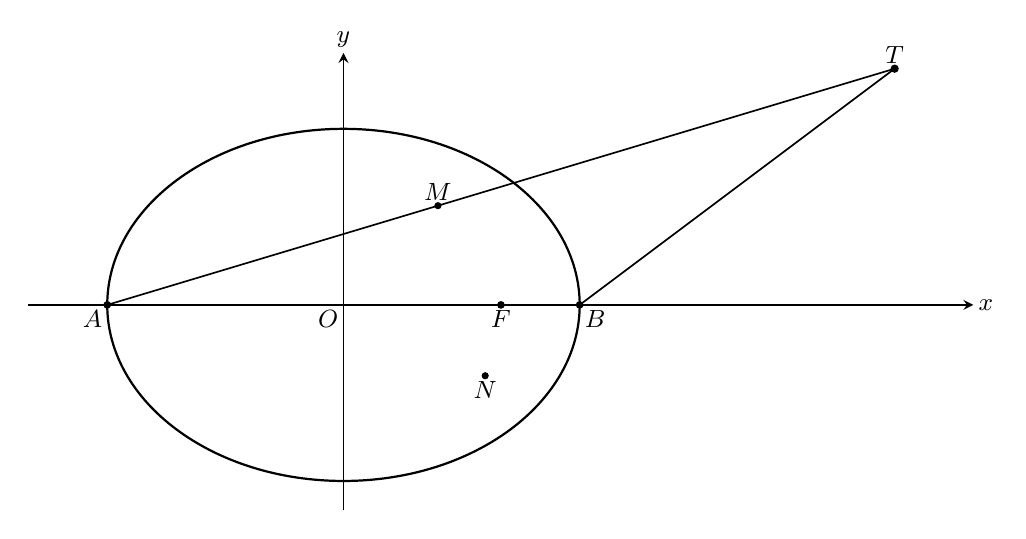
\begin{tikzpicture}[semithick, scale=1.0, every node/.style={inner sep=1.6pt, font=\small}]
  \draw[-stealth] (-4,0) -- (8,0) node[right] {$x$};
  \draw[-stealth] (0,-2.6) -- (0,3.2) node[above] {$y$};
  \draw[thick] (0,0) ellipse (3 and 2.236);
  \fill (-3,0) circle (1.4pt) node[below left] {$A$};
  \fill (3,0) circle (1.4pt) node[below right] {$B$};
  \fill (2,0) circle (1.4pt) node[below] {$F$};
  \fill (7,3) circle (1.5pt) node[above] {$T$};
  \draw (7,3) -- (-3,0);
  \draw (7,3) -- (3,0);
  \fill (1.2,1.26) circle (1.3pt) node[above] {$M$};
  \fill (1.8,-0.9) circle (1.3pt) node[below] {$N$};
  \node[below left] at (0,0) {$O$};
\end{tikzpicture}
